\documentclass[12pt, a4paper, tocpage=plain]{abnt} % Fonte tamanho 12, papel A4, páginas do sumário sem o p.<número da página>

\usepackage[brazilian]{babel} % Gera datas e nomes em português com estilo brasileiro
\usepackage{hyperref} % Permite a criação de hyperlink no documento, como os links usados na referência
\usepackage[utf8]{inputenc} % Dá suporte para caracteres especiais como acentos e cedilha
\usepackage[T1]{fontenc}
\usepackage[alf]{abntcite} % Define o estilo de referência bibliográfica
\usepackage{graphicx} % Permite a utilização de imagens no documento
\usepackage[small]{caption} % Define as legendas das figuras com fontes menores do que o texto
\usepackage{pslatex} % Define que o formato da letra será Times New Roman
\usepackage{epigraph} % Permite a criação de epígrafes 
\usepackage{setspace} % Permite a definição de espaçamento entre linhas
\usepackage[top=3cm, left=3cm, right=2cm, bottom=2cm]{geometry} % Define as margens da folha

\setcounter{secnumdepth}{3} % Até três subsubsections numeradas
\setcounter{tocdepth}{3} % Até trẽs subsubsections numeradas

\setlength{\parindent}{1.25cm} % Define o recuo da primeira linha dos parágrafos para 1.25 cm

\usepackage{listings}
\usepackage{color}

\definecolor{dkgreen}{rgb}{0,0.6,0}
\definecolor{gray}{rgb}{0.5,0.5,0.5}
\definecolor{mauve}{rgb}{0.58,0,0.82}

\lstset{
  language=Python,% the language of the code
  numbers=left, %numeração de linhas à esquerda
  stepnumber=1,
  firstnumber=1,
  numberstyle=\tiny,
  extendedchars=true,
  frame=none,
  basicstyle=\footnotesize,
  stringstyle=\ttfamily,
  showstringspaces=false,
  captionpos=b,
  %language=Java, %deve ser definida na inclusão de cada trecho de código, 
  % pois podem existir linguagens diferentes em exemplos diferentes
  breaklines=true,
  breakautoindent=true,
  %estilos de comentário de uma e várias linhas
  keywordstyle=\color{blue},          % keyword style
  commentstyle=\color{dkgreen},       % comment style
  stringstyle=\color{mauve},         % string literal style
  frame=single,                   % adds a frame around the code
  extendedchars=\true,
  aboveskip=12pt,
  inputencoding=utf8,
}
\renewcommand{\lstlistingname}{Código}

\renewcommand{\ABNTchapterfont}{\bfseries} % Define a fonte do \chapter
\renewcommand{\ABNTchaptersize}{\large} % Define o tamanho da fonte do \chapter
\renewcommand{\ABNTsectionfontsize}{\large} % Define o tamanho da fonte da \section
\renewcommand{\ABNTsubsectionfontsize}{\large} % Define o tamanho da fonte do \subsection
\renewcommand{\ABNTsubsubsectionfontsize}{\large} % Define o tamanho da fonte do \subsubsection
\renewcommand{\ABNTbibliographyname}{REFERÊNCIAS BIBLIOGRÁFICAS} % Modifica o título gerado pelo \bibliographys

\begin{document} % Começo do TCC
\begin{titlepage}
 \begin{figure}[ht]
 \centering
 \scalebox{0.35}{
\includegraphics{figuras/logo}}
 \end{figure}
 \begin{center}
   {\large BACHAREL EM SISTEMAS DE INFORMAÇÃO} \\ [3.5cm]
   {\large PRISCILA MANHÃES DA SILVA} \\ [4cm]
   {\large DESENVOLVIMENTO DE NOVAS FUNCIONALIDADES PARA A FERRAMENTA DE MANIPULAÇÃO DE ARQUIVOS EM NUVEM} \\
   \vfill
   {\large Campos dos Goytacazes/RJ} \\
   {\large 2012}
 \end{center}
\end{titlepage} % Cria a capa
\begin{titlepage}
 \begin{figure}[ht]
 \centering
 \scalebox{0.35}{
\includegraphics{figuras/logo}}
 \end{figure}
 \begin{center}
   {\large BACHAREL EM SISTEMAS DE INFORMAÇÃO} \\ [3.5cm]
   {\large PRISCILA MANHÃES DA SILVA} \\ [4cm]
   {\large DESENVOLVIMENTO DE NOVAS FUNCIONALIDADES PARA A FERRAMENTA DE MANIPULAÇÃO DE ARQUIVOS EM NUVEM}\\ [2cm]
   \hspace{.45\textwidth} % posicionando a minipage
   \begin{minipage}{0.5\textwidth}
   \begin{espacosimples}
        Trabalho de conclusão de curso apresentado ao Instituto Federal Fluminense como requisito obrigatório para obtenção de grau em Bacharel de Sistemas de Informação.\\[1.5cm]
        Orientador: Prof. Rogério Atem Carvalho\\
        Co-orientador: Prof. Fernando Carvalho
    \end{espacosimples}
    \end{minipage}
   \vfill
   {\large Campos dos Goytacazes/RJ} \\
   {\large 2012}
 \end{center}
\end{titlepage}
 % Cria a folha de rosto
\begin{folhadeaprovacao}
    \setlength{\ABNTsignthickness}{0.4pt}
    \setlength{\ABNTsignwidth}{15cm}
    \setlength{\ABNTsignskip}{0.9cm}
    \begin{center}
        {\large PRISCILA MANHÃES DA SILVA} \\ [4cm]
        {\large DESENVOLVIMENTO DE NOVAS FUNCIONALIDADES PARA A FERRAMENTA DE MANIPULAÇÃO DE ARQUIVOS EM NUVEM}\\ [2cm]
        \hspace{.45\textwidth} % posicionando a minipage
        \begin{minipage}{0.5\textwidth}
        \begin{espacosimples}
        Trabalho de conclusão de curso apresentado ao Instituto Federal Fluminense como requisito obrigatório para obtenção de grau em Bacharel de Sistemas de Informação.\\\\
        \end{espacosimples}
        \end{minipage}
    \end{center}
    Aprovada em 22 de novembro de 2012 \\\\
    Banca avaliadora:
    \assinatura{Prof. Rogério Atem Carvalho (Orientador) \\ Doutor em Ciências de Engenharia / IFF Campus Campos \\ Instituto Federal de Educação, Ciência e Tecnologia Fluminense / Campus Campos Centro}
    \assinatura{Prof. Fernando Luiz de Carvalho Silva (Co-Orientador) \\ Mestre em Engenharia de Produção / UENF \\ Instituto Federal de Educação, Ciência e Tecnologia Fluminense / Campus Campos Centro}
    \assinatura{Prof. Fábio Duncan de Souza \\ Mestre em Pesquisa Operacional e Inteligência Computacional / UCAM Campos \\ Instituto Federal de Educação, Ciência e Tecnologia Fluminense / Campus Campos Centro}
\end{folhadeaprovacao}
 % Cria a folha de aprovação
\null
\vfill

{\normalsize \it \hfill Dedico este trabalho à minha mãe e amigos por todo apoio, compreensão \vspace*{4pt}

\hfill e contribuição que me prestaram.}  % Cria a folha de dedicatória
\begin{center}
\textbf{AGRADECIMENTOS}
\end{center}

Primeiramente agradeço a minha mãe que sempre esteve ao meu lado nestes longos anos. \\
Agradeço também a todos meus amigos e colegas de trabalho do NSI, que me apoiaram e incentivaram. \\
Bem como aos professores Rogério Atem e Fernando Carvalho que contribuiram muito para que esse projeto fosse realizado.
 % Cria a folha de agradecimentos
\null % o \vfill só funciona com o \null
\vfill
\epigraph{O computador não é mais o centro do mundo digital.}{Tim Cook} % Cria a epígrafe (onde se coloca um pensamento)
\begin{center}
\textbf{RESUMO}
\end{center}
\singlespacing

\noindent Este trabalho descreve o desenvolvimento de novas funcionalidades para uma ferramenta livre de manipulação de documentos em larga escala, com o objetivo de permitir a mesma adaptar-se na manipulação outros formatos de arquivos através do acréscimo de aplicações comuns à sistemas operacionais baseados em linux. Assim com esta integração a ferramenta que encontra-se em constante desenvolvimento sob responsabilidade da empresa francesa Nexedi SA, com auxilio do Núcleo de Pesquisa em Sistemas de Informação(NSI-IFF), adquiriu a capacidade de manipular formatos correspondentes a arquivos de vídeo, áudio, imagens e PDF. Neste trabalho encontram-se ainda conceitos básicos empregados para formação da ferramenta e sua integração com o núcleo linux, bem como conceitos da linguagem Python, a qual foi utilizada para seu desenvolvimento. \\

\noindent PALAVRAS-CHAVE:  Serviço Web, Escalabilidade, Software livre, Python % Resumo do trabalho
\begin{center}
\textbf{ABSTRACT}
\end{center}

\singlespacing

\noindent This paper describes the development of new functionalities to a free tool of document manipulation on a large scale in order to allow it to adapt in handling other file formats through the addition of common applications for Linux-based operating systems. So with this integration tool that is constantly evolving under the responsibility of the French company Nexedi with the aid of the Nucleus of Research in Information Systems (NSI-IFF), acquired the ability to manipulate shapes corresponding to video files, audio, images and pdf. In this work are still used for training basic concepts of the tool and its integration with the core linux, as well as concepts of Python, which was used for its development. \\

\noindent KEYWORDS: Web Service, Scalability ,Free software ,Python
 % Resumo em língua estrangeira
\renewcommand{\listfigurename}{LISTA DE FIGURAS} % Modifica o nome da lista de figuras
\listoffigures % Gera o índice de figuras
\renewcommand{\contentsname}{SUMÁRIO} % Modifica o nome do sumário
\tableofcontents % Gera o sumário
\onehalfspacing % Define o espaçamento de 1.5cm entre linhas
\chapter{INTRODUÇÃO}
\thispagestyle{empty}

Segundo \cite{TESLA}, a Internet é um produto descendente de um experimento militar americano que tentava formar uma rede que não fosse vulnerável ao ataque inimigo, e que desde seu processo de desmilitarização expandiu ao redor mundo, mesmo em continentes afastados e pouco populosos como a Antártica.  

Ela foi fundamental para criação do \textit{Cloud computing}, em português computação nas nuvens, que consiste em permitir ao usuário acesso a diversas aplicações e ao máximo de funcionalidades que esta nova forma de interação entre maquina e usuário possa disponibilizar, independente da plataforma em que o mesmo se encontre, tornando-se cada vez mais ampla a medida que o avanço tecnológico permite maior acesso a Internet.

Seguindo esta tendência, mesmo antes de sua popularização, o Núcleo de Pesquisa em Sistemas de Informação(NSI) já trabalha anos no desenvolvimento e melhoria do projeto Biblioteca Digital da RENAPI, o qual visa disponibilizar um acervo bibliográfico digital para disseminação de científico tecnológico produzido na rede de Instituições de Educação Profissional Científica e Tecnológica (EPCT).

Assim o NSI passou a utilizar, entre outras, a ferramenta \textit{OpenOffice.org Daemon}, a qual foi desenvolvida originalmente pela empresa francesa Nexedi SA. Essa ferramenta possuía por objetivo a conversão de documentos.

No entanto a partir do uso prolongado da mesma, foram identificados erros considerados em parte graves para uma aplicação desta extensão. Entre esses é possível citar perda de conexão, \textit{deadlock} no OpenOffice.org utilizado pela aplicação, estouro de memória entre outros.

Assim dada a necessidade de corrigir estes erros a fim de obter estabilidade, através da parceria do NSI com a Nexedi,foi realizada a analise desta ferramenta.

Entretanto a análise provou que era inviável corrigir tal ferramenta em função de novas demandas também percebidas.

Definiu-se assim uma nova meta, a proposta da criação de uma ferramenta que fosse capaz de manter as conversões desta, mas que tivesse seus principais erros corrigidos, e que ainda fosse capaz de extrair e manipular informações pertencentes aos documentos em questão.

Em 2010, a ferramenta Web Service OOOD 2.0 foi apresentada. Seguindo em parte a sigla da antecessora, esta correspondia as expectativas implícitas na ultima analise realizada, no entanto, dado que os objetivos anteriores foram alcançados, e com base no aprendizado envolvido neste desenvolvimento, novas metas foram traçadas.

Além de poder manipular documentos tornou-se desejável também que a ferramenta fosse capaz de manipular arquivos de imagem, vídeo, áudio e PDF.

\section{Objetivo}

Este trabalho tem como principal objetivo apresentar a ferramenta sucessora ao OOOD 2.0, com intuito de demonstrar suas atualizações e ampliações. O CloudOoo provou-se capaz de manipular outros formatos de arquivos, ainda que prematuramente não tenha mesma estabilidade, mas que caminha para isto.

\section{Estrutura do trabalho}

Este trabaho se divide em cinco capítulos a partir deste primeiro:

O segundo capítulo deste trabalho cita e explica sobre as principais ferramentas que permitiram ao CloudOoo alcançar os objetivos inicialmente traçados, e que estão diretamente envolvidas a este, demonstrando um pouco sobre cada uma delas.

No terceiro capítulo é apresentada a nova estrutura sobre a qual o CloudOoo vem sendo desenvolvido, e sobre sua necessidade para seu funcionament.

No quarto capítulo é apresentado um breve estudo de caso do desenvolvimento desta ferramenta, avaliando seu desenvolvimento; falando sobre aplicações que o utilizam e demonstrando sobre sua atual estabilidade com base em estudos anteriores.

Por fim no quinto capítulo são apresentadas as conclusões sobre este trabalho e de proposta futuras para a melhoria desta ferramenta.

\chapter{CONCEITOS BÁSICOS}

Este capítulo apresenta um conceito simplifica sobre cada ferramenta utilizada para o desenvolvimento desta aplicação, ou que utilize a mesma.

\section{Python}

Python é uma linguagem de programação poderosa e fácil de aprender. Tem estruturas eficientes e de alto nível de dados além de uma abordagem simples, entretanto eficaz para programação orientada a objeto. Sua sintaxe elegante, de tipagem dinâmica, juntamente com a sua natureza interpretada, tornam-na uma linguagem ideal para \textit{scripts} e desenvolvimento rápido de aplicações em muitas áreas, na maioria das plataformas \cite{GUIDO}.

\subsection{Buildout}

\textit{Buildout} é uma ferramenta desenvolvida em python, capaz de criar um ambiente isolado para desenvolvimento de novas aplicações. Ele fornece suporte para criação diversas aplicações, especialmente em Python, mas não somente. Fornece ainda ferramentas para montagem de receitas para aplicações de múltiplas partes. Uma única aplicação pode conter vários programas, processos e definições de configuração \cite{BRANDOM}.

Levando em consideração o ideal do ambiente separado, também chamado de puro, a instalação do \textit{buildout} é extremamente simples a partir de um arquivo de \textit{script} python, que ao ser executado gera um segundo \textit{script} 'bin/buildout' e a partir deste toda aplicação pode ser gerada com base no arquivo de configuração como da Figura \ref{buildout}:

\begin{figure}[ht]
    \centering
    \scalebox{0.7}{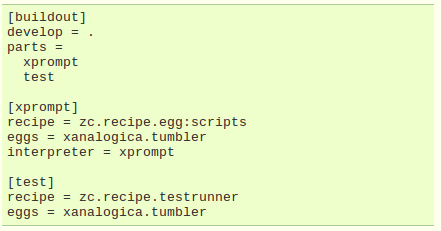
\includegraphics{figuras/buildout}}
    \caption{Simples módulo buildout.cfg. Adaptado de \cite{ZOPE-FOUNDATION-BUILDOUT}}
    \label{buildout}
\end{figure}

A descrição superior \textit{[buildout]} é a única realmente obrigatória para identificação de um arquivo de configuração. Na segunda linha definimos que o diretório em que o arquivo se encontra será um local de desenvolvimento da aplicação, nas três seguintes estão definidas suas partes, ou seja, a ordem em que cada parte, seja uma operação ou aplicação acoplada, será executada.

O \textit{recipe} trata-se do componente responsável pela parte a qual é citado. \textit{Egg} trata-se da opção referente as dependências de cada parte e por fim \textit{interpreter} representa ao \textit{buildout} que deseja-se um interpretador python contendo as dependências desta parte e que seja renomeado para \textit{xprompt}.


Ainda que incomum, volto a ressaltar que aplicações não desenvolvidas em python podem ter seu ambiente gerado pelo \textit{Buildout}, basta mudar algumas especificações e ter de fato o python instalado como dependência do \textit{buildout} e não da aplicação desejada.

\subsection{Subprocess}

O \textit{subprocess} é um modulo python que permite a aplicação expandir processos executados pelo \textit{shell}, ou que transmita-se informações de entrada, saída e erro de aplicações. Este módulo foi criado na intenção de substituir outros módulos e funções obsoletas, além de permitir também maior iterabilidade entre a aplicação e o sistema no qual se encontra.

\begin{figure}[ht]
    \centering
    \scalebox{0.7}{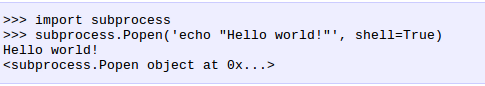
\includegraphics{figuras/subprocess}}
    \caption{Exemplo de uso do shell pelo subprocess. Adaptado de \cite{GADNER-SUBPROCESS}}
    \label{subprocess}
\end{figure}

Na Figura \ref{subprocess} existe um pequeno exemplo de como o \textit{subprocess} pode ser utilizado, neste exemplo ele é utilizado para acessar o \textit{shell}, como pode ser verificado no final da segunda linha em 'shell=True', e demonstrar um \textit{Hello World} através do comando \textit{echo}.

Em aplicações que utilizam outros ambientes isolados, ou seja, sem demais instalações, como citado na sessão anterior \ref{buildout}, é preferêncial que a variável \textit{shell} tenha valor \textit{false} na chamada da função a fim de usar as aplicações criadas neste ambiente,porém este é o valor padrão para esta variavél, assim não é preciso declará-lo, como por exemplo no código \ref{codigo_subprocess_convert}.

\begin{figure}[ht]
    \centering
    \scalebox{0.7}{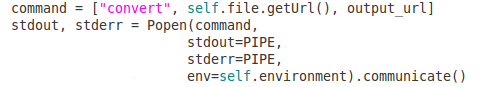
\includegraphics{figuras/subprocess_convert}}
    \caption{Exemplo de uso subprocess do CloudOoo}
    \label{subprocess_convert}
\end{figure}

Embora tenha uma descrição um pouco mais complexa, esta figura esta representando uma chamada do \textit{subprocess} em que utiliza-se o comando \textit{convert}, utiliza-se a opção \textit{PIPE} para que, após executado, o comando retorne as mensagens de saída e erro respectivamente através das variáveis \textit{stdout} e \textit{stderr}. Além disso na chamada também utiliza-se a variável \textit{env} a fim de informar a aplicação caminhos para binários que estão em seu ambiente de desenvolvimento.

Assim sendo, o \textit{subprocess} pode ser considerado um dos melhores módulos python para trabalhar com ambientes isolados.

\subsection{Zope}

Zope (Z Object Publishing Environment) é uma serviço web livre de código aberto desenvolvida em python \cite{ZOPE2}.

Zope já foi considerada a aplicação que popularizou o python, Não existiu ferramenta em Perl que o levasse as pessoas como o Zope levou o python \cite{UDELL}, no entanto se tornou muito extensa e complexa, com alto nível de taxa de aprendizagem, sendo mais tarde ofuscada pela ferramenta Djando em questão de popularidade. Mas essa expansão resultou na criação de vários produtos independentes que continuam facilitando na construção de aplicações python.

\subsubsection{Zope Interfaces}

Como citado na sessão anterior, diversos pacotes Zope foram criados individualmente com intuito de auxiliar na criação de outras aplicações python, de forma a não deixá-la muito extensa ou pesada, entre elas a \textit{zope.interface} é uma aplicação independente escrita em python e mantida pela equipe Zope.

O \textit{zope.interface} foi criado com intuito de permitir a comunicação entre qualquer componentes externos que possuissem uma \textit{Application Programming Interface} (API). A ideia de criar uma interface para os componentes de uma aplicação é uma forma quase elegante de resolver um antigo problema de tipagens dinâmicas tratando as informações recebidas de forma genérica, a fim de renderizá-las para um tratamento mais específico.

\section{XML}

O \textit{Extensible Markup Language} (XML) é um formato de texto simples para representação de informações sobre estruturas: documentos, dados, configurações, livros, transações, faturas entre outros. Foi derivado de um formato antigo chamado SGML (ISO 8879), para ser mais flexível ao uso Web \cite{W3C-XML}.

Atualmente se tornou um dos formatos mais comuns para compartilhamento de informações em aplicações web, por ser simples de ser escrito e corresponder a um padrão comum ao HTML, que por muitos anos já vem sendo utilizado pelas mesmas.

Além disso este formato dispõe de outras vantagens como: padrão de \textit{markup}, cujo o nome é detalhado de forma redundante; a descrição da estrutura de forma geral também permite uma compreensão de código bem literal, como se fossem textos; todas suas versões são capazes de processar e ler qualquer documento XML, mesmo que algumas delas procurem por \textit{markups} específicos.

\section{Formato Aberto}

O formato aberto é uma especificação publicada para armazenar dados digitais, mantido geralmente por uma organização de padrões não proprietária, e livre de limitações legais no uso.

Um formato aberto deve ser tanto implementável em software proprietário quanto software livre, usando as licenças tipicas de cada um. Em contraste com o formato proprietário que é controlado e defendido por interesses particulares da empresa detentora de seus direitos. O objetivo principal dos formatos abertos é garantir o acesso a longo prazo aos dados sem incertezas atuais ou futuras no que diz respeito às diretas legais ou à especificação técnica. Um objetivo secundário dos formatos abertos é permitir a competição, em vez de permitir que o controle de um distribuidor sobre um formato proprietário iniba o uso de um produto de competição.

\subsection{Formatos de Documentos}

Embora não seja considerado o formato ideal para documentos uma vez que não possui opções de formatação; tais como itálico e negrito, o \textit{.txt} é o formato aberto mais comum para arquivos de texto por ser pequeno e na maioria dos casos dispor de vários programas de edição.

Em 01 de maio de 2005, surgiu o \textit{OpenDocument Format}(ODF), um conjunto de formatos para aplicações de escritório com o objetivo de padronizar os formatos abertos. Seu nome original era \textit{Open Document Format for Office Application}, uma iniciativa da \textit{Organization for the Advancement of Structured Information Standards}(OASIS) em cima da base XML criada por desenvolvedores do OpenOffice.org, na época uma das poucas aplicações capazes de utilizar sua estrutura.

Atualmente os formatos ODF existem a 7 anos e foram adotados por diversas aplicações, entre elas a Microsoft Office, da Microsoft, mesmo sendo um software originalmente proprietário através de um \textit{pluggin} ele permite a edição e manipulação destes formatos.

Através da figura \ref{crescimento_odf} é possível acompanhar o crescimento do uso do ODF até 2010, ano em que fez 5 anos.

\begin{figure}[ht]
    \centering
    \scalebox{0.7}{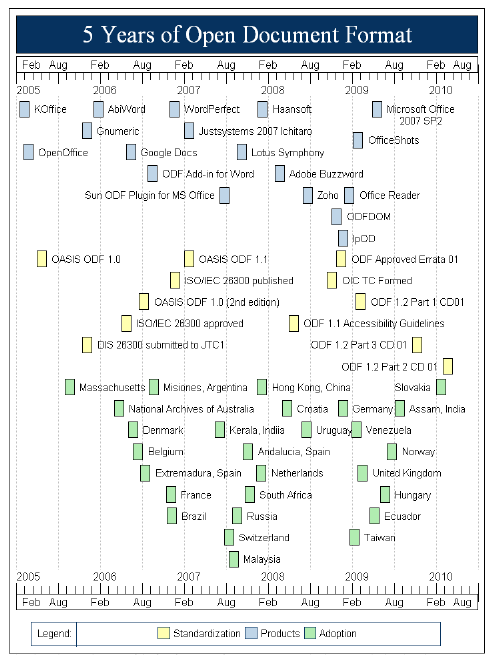
\includegraphics{figuras/crescimento_odf}}
    \caption{Crescimento do ODF nos primeiros cinco anos. Adaptado de \cite{SILVA}}
    \label{crescimento_odf}
\end{figure}

\begin{citacao}
O OpenDocument Format ainda é uma incógnita à grande maioria dos usuários comuns, mas sua adoção cresce em várias partes do mundo, especialmente nos meios corporativos e governamentais. No Brasil, por exemplo, o ODF já conta inclusive com aprovação da Associação Brasileira de Normas Técnicas (ABNT), que aconteceu em 2008 (norma NBR ISO/IEC 26300)\cite{ALECRIM-ODF}.
\end{citacao}

\subsubsection{Formatos de documentos ODF}

Embora exista um único padrão para identificação da estrutura de um ODF, como citado anteriormente, existem diversas extensões para o mesmo, como é possível observar na figura \ref{extensoes_odf}:

\begin{figure}[ht]
    \centering
    \scalebox{0.7}{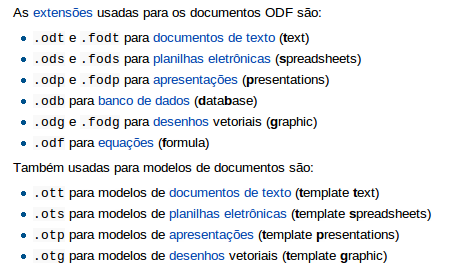
\includegraphics{figuras/extensoes_odf}}
    \caption{Extensões do ODF. Adaptado de \cite{WIKIPEDIA-ODF}}
    \label{extensoes_odf}
\end{figure}

Além destas extensões, é possível que arquivos ODF possam ainda utilizar da extensão de arquivo comprimido ZIP, outra opção de formato aberto só que para diversos arquivos a fim de diminuir seu tamanho.

\subsubsection{Estrutura de documentos ODF}

Sendo o ODF um conjunto de formatos abertos padrão, ele é constituído de uma estrutura única a fim de que toda e qualquer aplicações que o manipule obedeça seu padrão e permita que futuramente ele possa ser reutilizado por outra aplicações ou mesmo para permitir a extração de seus dados.

Esta estrutura é composta principalmente por:

\begin{itemize}
    \item{mimetype: arquivo de linha única constituído pelo mimetype do documento;}
    \item{content.xml: arquivo que armazena o conteúdo criado pelo usuário do documento;}
    \item{meta.xml: arquivo responsável por armazenar os \textit{metadados} do documento, ou seja, dados como autor, data de criação, data de modificação e outros;}
    \item{styles.xml: arquivo que contém os estilos do documento, tais como formatações de texto, parágrafos e outros;}
    \item{Pictures: pasta que armazena figuras existentes no documento.}
\end{itemize}

Existem ainda diversos arquivos e pastas que podem compor um documento ODF para compor o arquivo final, assim pode-se concluir que estes formatos representam uma diferente linha de arquivos comprimidos.

\subsection{Formatos de Imagens}

No que desrespeito a imagens a questão livre trata sobre patentes dos formatos, ou inclusa neles.

Assim em 1996 surgiu o formato \textit{Portable Network Graphics}(PNG) que tinha como principal objetivo substituir o formato GIF, portador de inúmeros algoritmos patenteados.

O PNG é um formato livre, criado desde o início para ser utilizado em qualquer aplicação sem necessidade de pagamentos de licenças ou afins.

Além disso este formato permite comprimir imagens sem perda de qualidade e também a retirada do fundo de imagens através do canal alfa; possui suporte de milhões de cores, diferentemente do GIF, cujo suporte era de 256 cores; e ainda permite a criação de animações, cujas extensões podem variar em \textit{.mng} e \textit{.apng}, mas são igualmente livres.

Este é apoiado pela \textit{World Wide Web Consortium}(W3C) e o único formato realmente livre existente no momento, e em 2003, mesmo ano em que a patente do formato GIF expirou, tornou-se padrão internacional.

\subsubsection{Estrutura do PNG}

Um arquivo PNG consiste de uma assinatura PNG e seguido de vários blocos em serie \cite{PNG-BOOK}.

Sua assinatura equivale aos primeiros oito \textit{bytes}, consiste da serie “137 80 78 71 13 10 26 10”.

Cada bloco consiste de:

\begin{itemize}
    \item{length: inteiro correspondente ao numero de \textit{bytes} dos dados da imagem;}
    \item{chunk type: código equivalente ao tipo do bloco;}
    \item{chunk data: dados da imagem;}
    \item{Cyclic Redundancy Check(CRC): campo que contém o valor total de \textit{bytes} do bloco, o \textit{chunk type} e o \textit{chunk data}, mas sem o valor do \textit{length}.}
\end{itemize}

O inicio da serie de blocos deve conter um \textit{IHDR chunk} e o ultimo bloco deve conter um \textit{IEND chunk} como \textit{chunk type} sinalizando que representam o inicio e fim da serie respectivamente.

\subsubsection{Exif}

O \textit{Exchangeable Image File Format}(Exif) é um conjunto de \textit{metadados} a respeito da imagem em questão, ou seja, são dados como autor, dia em que a foto foi tirada, câmera utilizada, entre outros listados conforme um padrão.

Todas essas informações ficam dentro da própria imagem, no entanto é preciso ter uma aplicação especifica para vê-lo, e em casos de informações mais abrangentes, as vezes é necessário possuir também uma aplicação para manipular a imagem e inserir nela \textit{metadados} a respeito da imagem.

\subsection{Formatos de Áudio}

Os formatos livres de áudio tratam sobre codecs disponíveis sem uma patente aplicada aos mesmos. Nesta categoria conta-se com os formatos de \textit{Vorbis}(OGG) e \textit{Free lossless Áudio Codec}(FLAC).

O FLAC é um formato livre de áudio comprimível e sem perda de qualidade e dados durante a o processo de compreensão. Seu algoritmo permite que o arquivo reduza em até 60\% seu tamanho original, e também permite a manipulação de \textit{metadados}.

OGG Vorbis é um novo formato comprimível de áudio É grosseiramente comparado com outros formatos utilizados para guardar e reproduzir musicas, tais como MP3, VQF, AAC, e outros formatos de áudio digital. Mas é diferente de todos estes formatos porque é livre, aberto e sem patentes \cite{XIPH}.

\subsection{Formatos de Vídeo}

Assim como os arquivos de áudio, a licença dos formatos de vídeo tratam sobre patentes de codecs, e neste caso as extensões mais comuns são conhecidas por \textit{Theora}(OGV) e \textit{Matroska}(MKV).

Theora é de proposito geral, um codec de vídeo com perda de dados. É baseado no codec de vídeo VP3 produzido pela On2 Tecnologies \cite{XIPH-THEORA}.

Matroska é o nome de uma iniciativa ousada para a criação de formatos universais de contentores, ou \textit{containers} de áudio e vídeo digitais \cite{WIKIPEDIA-MATROSKA}.

Assim o MKV trata-se de um contentor de padrão aberto para vídeos, que pode conter vários dados de diferentes tipos de codificações.

\section{LibreOffice}

O LibreOffice é um pacote de software de produtividade compatível com a maioria dos softwares semelhantes, e esta disponível para varias plataformas. Ele é um software de código aberto e, por isso, é livre para baixar, utilizar e distribuir \cite{LibreOffice}.

Este pacote teve inicio em 2000, quando a Sun Microsystems liberou o código de seu produto StarOffice, e se chamava OpenOffice.org. Em 2010 a comunidade que desenvolvia o projeto anunciou a fundação independente \textit{The Document Foundation}, a fim de cumprir com a independência explicita da carta de inicio do projeto.

Assim no inicio de 2011 foi lançado o LibreOffice 3.3, que bem como o OpenOffice.org 2.0, já suportava a edição da suíte \textit{OpenDocument}.

\subsection{UNO}
\label{uno}

O projeto OpenOffice.org possui uma característica muito útil e pouco utilizada que é a capacidade de integrar seu funcionamento com outros aplicativos. Isto é possível através do UNO (Universal Network Objects), que é um modelo de componentes do OpenOffice.org.

O UNO oferece interoperabilidade entre diferentes linguagens de programação, diferentes modelos de objetos, diferentes arquiteturas e processos, em uma rede local ou mesmo através da internet. Seus componentes podem ser implementados e acessados por qualquer linguagem de programação que possua acesso aos \textit{bindings} do UNO \cite{MINETTO-PYUNO}.

Atualmente existem \textit{bindings} para as linguagens C, C++, Java e Python. Desde a versão 1.1 o OpenOffice.org dispõe do pyUNO em sua instalação por padrão.

\subsubsection{PyUNO}

O PyUNO representa uma ``ponte'' entre o LibreOffice e aplicações Python. Através dele é possível a manipulação do componente UNO, seção \ref{uno}, para utilizar praticamente todas funcionalidades disponíveis no LibreOffice por \textit{scripts} Python.

No entanto, segundo \cite{PYUNO}, essa ferramenta ainda não atingiu seu uso absoluto podendo conter diversos \textit{bugs}, e assim dependendo em grande parte de coloboração por parte da comunidade que utiliza a mesma.

Na Figura \ref{exemple_uno} é possível ver um exemplo pratico do uso do PyUNO em um código python:

\begin{figure}[ht]
    \centering
    \scalebox{0.7}{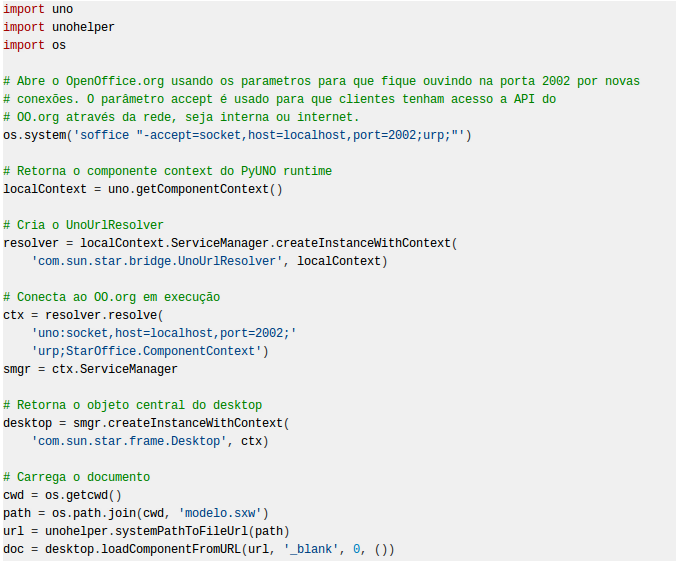
\includegraphics{figuras/exemple_uno}}
    \caption{Exemplo de uso do UNO com python(PyUNO). Adaptado de \cite{MINETTO-PYUNO}}
    \label{exemple_uno}
\end{figure}

Nela é possível observar passo a passo o código python, atentando aos comentários, neste exemplo ele utiliza o LibreOffice em \textit{localhost}, ou seja, suas modificações são apenas realizadas na própria maquina, no entanto, no caso de um serviço web é possível passar o endereço do mesmo e alterar a porta utilizada para estabelecer comunicação.

\section{ImageMagick}

ImageMagick é uma suíte de aplicações para criar, editar,compor ou converter imagens \textit{bitmap} \cite{IMAGEMAGICK-STUDIO}.
Na realidade o ImageMagick disponibiliza um conjunto de binários, compatíveis com varias plataformas, que no Linux são dados como comandos separados para diversas funcionalidades.

Para \cite{TESLA} é uma ferramenta, originalmente criada por John Cristy, para visualizar e manipular imagens, que esta amplamente disponível na Internet.

As funcionalidades que podem ser consideradas mais comuns e utilizadas são \textit{convert} e \textit{identify}, essas funcionalidades podem respectivamente: converter imagens para outros formatos ou formatação, como invertido ou de girar em 180 graus; e identificar os \textit{metadados} disponíveis na imagem, como autor, ou data que foi criada ou tirada.

\section{XPDF}

Xpdf é uma ferramente de código aberto para visualização de arquivos Portable Document Format(PDF) \cite{GLYPH-COG}.

Além de permitir a visualização de arquivos PDF o \textit{xpdf} é uma ferramenta que permite a extração de textos dentro destes formatos de arquivos e a conversão dos mesmos para \textit{postscript}, formato de arquivos especialmente compostos de informações e desenvolvido originalmente pela \textit{Adobe System}.

Assim como a maioria das aplicações para Linux é utilizada através de comandos, neste caso o mais comum \textit{pdftotext} o qual captura o texto disponível no arquivo PDF e passa para aplicação que o utilizou em forma de texto simples.

\subsection{Poppler}

O poppler é uma biblioteca para renderizar PDF baseada no xpdf 3.0 \cite{JOHNSON}.

É uma das bibliotecas de código livre mais utilizada pelos sistemas Linux para leitores PDF, seu desenvolvimento é idealizado pela FreeDesktop.Org.

\section{PDFTk}

Se o PDF é um trabalho eletrônico, então o pdftk é o removedor de grampo, furador, pasta, anel decodificador secreto e o óculos de raio-X. Pdftk é a ferramenta simples para fazer as tarefas de todos os dias com documentos PDF \cite{STEWARD}.

Esta ferramente esta sob licença GPL e utiliza bibliotecas que possuem suas próprias licenças de uso.

Na realidade de simples o \textit{pdftk} tem apenas seu uso, é uma ferramenta de fácil utilização, que no entanto permite a livre manipulação de documentos PDF, criado pelo autor do livro “PDF Hacks”, Sid Steward, é considerada uma ferramenta profissional.

\section{FFMPEG}

Para \cite{FFMPEG-SCALABLE}, a melhoria constante do uso do processamento de multimédia, requerida e obtida pela expansão multifuncional e acelerada dos equipamentos de hardware, requer também aplicações eficientes e escaláveis a medida que este processo avança. E partindo deste principio uma das ferramentas ideias para projetos escaláveis é o FFMPEG.

Ffmpeg é um rápido conversor de vídeo e áudio que também consegue tratar informações momentâneas de ambos. Ele também pode converter faixas arbitrarias de amostras e redimensionar vídeos através de filtros polifásicos de alta qualidade \cite{FFMPEG}.

Mais do que isso, o \textit{ffmpeg} é uma suíte de aplicações via linha de comando capaz de converter, extrair e inserir \textit{metadados} em arquivos de áudio e vídeo de simples entendimento, de fácil uso.

\section{SERVIÇOS WEB}

Segundo \cite{Pirnau-Apetrei-Badea}, os serviços web representam a metodologia em que aplicações podem se comunicar através de mensagens assíncronas ou chamadas remotas. Assim pode se dizer que serviços web são aplicações acessáveis remotamente.

Toda empresa tem por objetivo prover serviços, sejam esses para própria empresa, ou para clientes, que por sua podem ser outras empresas. A anos esses serviços têm sido automatizados, inicialmente aplicações \textit{desktop} eram criadas quando a empresa era pequena e possui poucas maquinas, ou a comunicação entre elas não era tão necessária.

Quando a rede passou a estar presente no dia a dia de forma geral essas aplicações foram evoluindo e buscando a comunicação entre as mesmas.

Este conceito na verdade trata da iniciativa por parte dessas empresas de retirar suas aplicações da maquinas próprias e passá-las para potente servidores que disponibilizarão esta na internet, assim basta ter acesso a internet e é possível utilizar esta aplicação.

\section{XML-RPC}

É um protocolo para chamadas remotas que utiliza HTTP para transporte e XML para encodificação. O XML-RPC foi desenhado para ser o mais simples o possível, enquanto permite que uma estrutura de dados complexa seja transmitida, processada e retornada \cite{XMLRPC}.

Foi originalmente criado por Dave Winer na UserLand Frontier, e inspirado por outros dois protocolos, um também desenvolvido pelo próprio Dave Winer e outro que representava o começo do protocolo SOAP. Entretanto seu uso é bem mais simples de se utilizar e entender que o SOAP. Suas mensagens correspondem a uma requisição HTTP-POST, enquanto composição do corpo da mensagem é escrita em XML, bem como a resposta que a requisição recebe.

\section{WSGI}

O \textit{Web Service Gateway Interface}(WSGI) é uma Interface de entrada para serviços web. É uma especificação para serviços e aplicações web para que haja comunicação com outras aplicações web(embora possa ser utilizada para outras funções). É um padrão Python, escrito sob a PEP 333 \cite{WSGI}.

Esta interface foi escrita com o objetivo de fornecer uma forma relativamente simples e compreensiva de comunicação entre aplicações e servidores, ou pelo menos com a maioria das aplicações web em python, e que ainda pudesse suportar componentes \textit{middleware}.

\subsection{Paster}

O \textit{Paster} se trata de um servidor web, composto pelo \textit{Python Paste}, que segue o padrão da interface python WSGI.

Possui dois níveis de linha de comando composto inicialmente por \textit{paster}, onde o segundo comando especifica o serviço desejado, como \textit{serve} no caso de estabelecer o servidor, seguindo como parâmetros o restante das informações necessárias para estabelecer o serviço desejado.

É considerado um dos mais simples servidores web para python, no entanto pode ser utilizado assincronamente e manter uma escalabilidade considerável até 2000\textit{rps}.

\section{Git}

Git é um sistema de controle de versão distribuída livre e de código aberto, projetado para lidar com qualquer projeto, desde o menor ao maior com rapidez e eficiência \cite{SOFTWARE-FREEDOM-CONSERVANCY}.

A historia do Git está muito relacionada a criação do Linux e de seu criador Linus Torvalds, bem como com toda comunidade de desenvolvimento Linux. Durante anos a comunidade utilizou a ferramenta \textit{BitKeeper} para guardar a modificações do projeto.

Em 2005, após um problema com a proprietária deste, a comunidade decidiu criar sua própria ferramenta a partir da experiencia com a anterior, houve um novo foco em: velocidade, \textit{design} simples, suporte para desenvolvimento paralelo, distribuição completa e a habilidade necessária para lidar com projetos grandes sem perda de velocidade e dados.

Assim, esse novo sistema de versionamento permite que qualquer repositório seja o centro do versionamento, deixando todo \textit{log} das modificações guardados nele sem que para isso precise de uma conexão a rede ou servidor geral.

\subsection{Git e Subversion}

Diferentemente do \textit{git}, o \textit{subversion} é um sistema de controle de versões centralizado, ainda muito utilizado atualmente, principalmente por projetos livres.

Embora seja consideravelmente rápido, é extremamente desaconselhável para projetos grandes e principalmente desenvolvidos paralelamente.

\subsection{Biblioteca Digital}

A Biblioteca Digital da Rede Nacional de Pesquisa e Inovação(RENAPI), é um projeto que visa disponibilizar um acervo bibliográfico digital para contribuir com a disseminação de material científico e tecnológico produzido na rede de Educação Profissional Científica e Tecnológica(EPCT), sendo esse material periódicos, teses, monografias, artigos entre outros. Assim esse disseminação visa colaborar na qualificação do material humano digitalizado e na disseminação de conhecimento.

Este projeto é um dos principais desenvolvidos no Núcleo de Pesquisa em Sistemas de Informação(NSI), que conta atualmente com ??? bolsistas e ??? pesquisadores.

\subsection{ERP5}

Um ERP é capaz de integrar processos e dados de uma organização, através de recursos tecnológicos que padronizam e automatizam os mesmos.

Muito seja um sistema propriamente dito, ele foca mais em processos do que em funcionalidades, ele mascará informações em funcionalidades transparentes(\cite{PITRE-DESAI}).

No entanto, apesar de trazer muitas vantagens a organização, esse processo de automatização, de forma geral, é longo, de alto custo e complexidade, e até mesmo difícil de implementar.

De acordo com \cite{SMETS-CARVALHO}, esta situação que motivou a criação do ERP5, cujas ferramentas são de código aberto, permitindo que a organização modifique-o a fim de torná-lo mais flexível aos seus processos.

Ele também incorpora conceitos avançados como o de banco de dados orientados a objetos, um sistema de gerenciamento, de sincronização, variação, \textit{workflows}, e possibilita a implementação de \textit{Business Templates}.

Compreende-se assim o ERP5, como sendo um ERP de baixo custo de implantação e alta tecnologia para pequenas e médias empresas.

\subsection{SlapOS}

O SlapOS é um sistema operacional de código aberto para o uso de redes distribuídas em computação em nuvem, que se baseia em que tudo se trata de um processo.

Para \cite{SMETS-CERIN-COURTEAUD} a computação em nuvem é dividida em três camadas, infra-estrutura como serviço (IaaS), Plataforma como Serviço (PaaS) e Software como Serviço (SaaS). Na IaaS esta o funcionamento virtual da maquina e seu armazenamento, sob o ele é construido o Paas, que funciona como coração dos serviços, como servidor e bancos de dados. Finalmente sobre Paas estão as aplicações de uso do usuário.

Através de uma API unificada e simples, que requer poucos minutos para aprendizagem, este sistema combina computação em grade e o conceito de ERP para fornecer estas categorias previstas na compução em nuvem.

Dada sua abordagem unificada e arquitetura modular, ele tem sido usado como uma ferramenta de testes para benchmark de bancos de dados NoSQL e para otimização do processo de alocação em nuvem.


\chapter{CloudOoo}

Em 2006, em função da necessidade da conversão de documentos a empresa francesa Nexedi SA originou a construção da ferramenta OpenOffice.Org Daemon (OOOD 1.0), com base no uso da ferramenta LibreOffice, para conversão de documentos, no entanto com o uso prolongado desta ferramenta, em ambientes de produção, foram identificados erros relacionados com a aplicação e com a sua atuação com o LibreOffice. Entre eles estavam erros como perdas de requisições, deadlock de processo, e no LibreOffice e memory leak.

Assim foi ressaltada a necessidade de modificações a fim de que a aplicação se tornasse mais estável, além de adicionar novas funcionalidades, como de exportar documentos para outras extensões além de ODF, PDF por exemplo, e também manipular informações destes, conhecidas como \textit{metadados}.

O resultado da continuação do desenvolvimento foi a ferramenta \texit{Web Service OOOD 2.0}, posteriormente nomeada por CloudOoo, apresentada em 2010. Esta nova versão da ferramenta se provou bem mais estável no uso a longo prazo, embora fosse considerada mais lenta em processos individuais, devido aos tratamentos adicionados para os erros conhecidos, e suas modificações de novas funcionalidades.

Ao final do processo de melhoria da ferramenta novas funcionalidades foram idealizadas para diferentes tipos de arquivos, como converter e manipular documentos, bem como arquivos de áudio, vídeo, imagem e PDF.

Assim o CloudOoo apresentado neste capítulo, é um serviço Web livre e de código aberto, sob a licença LGPL, que foi desenvolvido através parceria da Nexedi SA e do NSI, na linguagem de programação Python e que utiliza o protocolo XML-RPC para troca de mensagens, que pode ser utilizado inteiramente ou em partes separadas.

\section{Estrutura}

Desde de sua estrutura anterior, o CloudOoo foi desenvolvido para trabalhar de forma genérica prevendo futuras mudanças. Sua estrutura contém com estas interfaces:

\begin{itemize}
    \item{IApplication: representa os métodos de controles as aplicações externas do servidor;}
    \item{IFile: que representa métodos para manipulação de arquivos recebidos pelo servidor;}
    \item{IOdfDocument: representa métodos de manipulação de documentos ODF recebidos pelo servidor;}
    \item{IHandler: representa os objetos que irão realizar a requisição emitida pelo cliente;}
    \item{IMonitor: representa métodos de controle e manuseio dos processos estabelecidos no servidor;}
    \item{IMimemapper: representa métodos utilizados para trabalhar com filtros;}
    \item{IFilter: representa métodos de tratamento de filtros;}
    \item{ILockable: representa os métodos de controles criados para região crítica do servidor;}
    \item{ITableGranulator: representa métodos para extrair tabelas de documentos;}
    \item{IImageGranulator: representa métodos para extrair imagens de documentos;}
    \item{ITextGranulator: representa os métodos para extrair o conteúdo de um documento em capítulos e parágrafos;}
    \item{IERP5Compability: representa os métodos de compatibilidade com o ERP5;}
    \item{IManager: representa os métodos utilizáveis entre cliente e servidor.}
\end{itemize}

As próximas subseções apresentam detalhadamente sobre cada interface e as principais classes a implementá-las.

\subsection{IApplication}

Por possuir a opção de estar instalado num ambiente própria onde tanto o CloudOoo, assim como as ferramentas utilizadas pelo mesmo, podem possuir instalação própria a partir do uso do \textit{buildout}, foi preciso construir uma interface para controlar as funções dos processos utilizados pela aplicação, ou seja, uma classe que fosse capaz de carregar a configurações das aplicações, controlar a inicialização e finalização de cada processo, e que fosse capaz de verificar se continuavam rodando no sistema operacional, a partir de um identificador e/ou da porta que cada uma utilizasse.

\subsubsection{Application}
\label{application}

Esta classe implementa a interface IApplication e tem por objetivo controlar aplicações que estejam dentro do processo do cloudooo, como o LibreOffice que precisa estar executando para possibilitar a manipulação dos documentos.

Ela possui os métodos responsáveis por carregar as configurações, iniciar e parar o processo, igualmente o método de reiniciar a instancia, utilizado principalmente caso esta apresente algum erro durante processos; um método para verificar o status dessa aplicação através do método de \texit{pid} que retorna o pid utilizado pela aplicação.

Além desses métodos existe um responsável por endereço dessa aplicação, ou seja, onde esta estabelecida e em qual porta.

\subsection{IFile}
\label{ifile}

Esta interface propõe um contrato de tratamento de arquivos, a fim de assegurar uma resposta eficiente e consistente ao cliente. Nela são contidos métodos para que o conteúdo do arquivo seja guardada durante sua instanciação de forma no acontecimento de erros não previstos este possa ter seu conteúdo recuperado, ou mesmo restaurado a forma original.

\subsubsection{File}
\label{file}

Com base na implementação da interface IFile, esta classe possui métodos para manter qualquer arquivo recebido do cliente no sistema apenas durante o uso do mesmo. Ao receber um arquivo ela escreve o mesmo no disco, podendo assim recuperar seus dados, e obter informações do mesmo, como seu caminho por exemplo.

Após o uso e manipulação deste ela é instituída a removê-lo do sistema, como demais métodos de tratamento de arquivos temporários.

\subsection{IOdfDocument}

Embora muito similar a interface IFile, descrita na seção \ref{ifile}, neste caso o tratamento é especifica para arquivos do tipo ODF, dada sua complexidade de armazenamento e manipulação.

\subsubsection{Document}

Por se trata de uma aplicação livre o foco dos tipos de arquivos do CloudOoo é igualmente livre, assim sua estrutura é relativamente planejada para estes, e no caso de documentos ODF, sua estrutura complexa e compacta exigiu que diversas classes fossem criadas especificamente para estes. É o caso desta classe, em seus métodos existe por exemplo o \textit{getContentXml} responsável pela leitura da estrutura XML desses tipos de documentos.

Outro razão para existência dessa estrutura vem a ser o tempo maior de estudo de manipulação de documentos em função dos outros tipos de arquivos.

\subsection{IHandler}
\label{ihandler}

Esta interface foi especificamente criada para estabelecer o contrato entre as aplicações externas utilizadas pelo servidor em função dos pedidos do cliente no que desrespeito a manipulação direta do arquivo, como no caso da conversão por exemplo, bem como a extração e inserção de \textit{metadados} do mesmo.

Para as classe que implementam esta interface é recomendado o igual uso de objetos do tipo File, apresentado na seção \ref{file}, para manipulação dos arquivos utilizados nas mesmas.

\subsubsection{OOHandler}

Dado o nome o OOHandler é a implementação especifica de comunicação com o LibreOffice. Ao receber uma requisição que trata de documentos é gerada uma instancia desta classe para manipulá-lo.

\subsubsection{PDFHandler}

Da mesma forma ocorre entre a classe PDFHandler e os arquivos do tipo PDF. Ao ser recebido pelo Manager, este arquivo será tratado diretamente nesta classe.

\subsubsection{IMAGEMAGICKHandler}

No que se trata de ferramentas para imagens o ImageMagick é uma das melhores disponível a nível de comando, ela consegue inclusive manipular dados do tipo \textit{Exif}, que são \textit{metadados} referentes a imagens.

Assim com base na aplicação foi escolhido o nome para esta classe responsável pelos arquivos de imagem.

\subsubsection{FFMPEGHandler}

No que se trata de arquivos de vídeo e áudio existe a ferramenta FFMPEG que é capaz de manipular ambos e portanto representa a classe responsável por estas instancias.

Assim como as demais classes que implementam o IHandler, esta classe é capaz de manipular os \textit{metadados} desses arquivos, bem como convertê-los para determinadas extensões do mesmo tipo.

\subsection{IMonitor}

Esta interface foi desenvolvida principalmente com base nos erros anteriormente obtidos com o uso do LibreOffice, no entanto é importante para o sistema como um todo, seu uso estabelece controles sobre princípios básicos do sistema, como uso de memória, tempo de requisições, tempo de uso do processo, entre outros.

\subsubsection{Monitor}
Basicamente a classe Monitor funciona como uma simples implementação da IMonitor a fim de estabelecer os atributos principais, como por exemplo o tempo minimo entre a monitorações do sistema. As próximas subseções explicam detalhadamente sobre estes controles através da herança desta classe.

\subsubsection{MonitorMemory}
\label{monitormem}

Nas configurações do CloudOoo existem definições que podem ser modificadas de acordo com o sistema em que vai ser instalado, entre elas existe uma variável responsável pelo uso máximo de memória pelo LibreOffice.

A partir dessa definição, dada em \textit{megabytes}, essa classe monitora o uso da memória do sistema, assim caso esta chegue em seu limite máximo de uso, a aplicação é reinicia com intuito de limpar da memória mensagens trocadas e que não liberaram o uso da mesma, evitando assim o evento chamado \textit{memory leak}, o qual consiste no uso de toda memória do sistema.

\subsubsection{MonitorTimeout}
\label{monitortim}

Também entre as definições da subseção \ref{monitormem} existe uma variável responsável pelo tempo limite de execução de um determinado processo, caso este tempo seja excedido ocorre o que chamamos de \textit{timeout} e a aplicação é forçada a parar, sendo reiniciada posteriormente.

A utilidade desta limitação é dada pela ideia de que caso este tempo tenha excedido ocorreu algum erro durante o processo, provavelmente em função da resposta da aplicação, assim reiniciá-la pode resolvê-lo.

\subsubsection{MonitorSleepingTime}

Com intuito de poupar uso do sistema em momentos desnecessários esta classe foi criada para observar o momentos de inutilização da aplicação e após determinado tempo parar a mesma. Assim é possível economizar no uso de recursos, e disponibilizá-los para outras aplicações que possam vir a utilizar o mesmo.

\subsubsection{MonitorRequest}

A fim de conservar a estabilidade do CloudOoo, esta classe implementa um controle em função do valor máximo de requisições que podem ser respondidas por cada instancia da aplicação, bem como nas subseções \ref{monitormem} e \ref{monitortim} a variável de reaquisições limite é estabelecido nas configurações.

Caso o valor informado seja excedido a instancia é parada e encerrada, em seguido uma nova instancia da mesma aplicação é iniciada.

\subsection{IMimemaper}

Em casos de aplicações como o LibreOffice que representam uma suíte de menores utilitários é preciso reconhecer a extensão de arquivo especifica para cada utilitário. De forma geral estas extensões são explicitas no nome do arquivo, entretanto no caso de que esta não esteja explicita é preciso reconhecer o tipo de arquivo de alguma outra forma. Neste caso existem o \textit{mimetypes}, que são identificações presentes no conteúdo do arquivo, que permitem decidir sua extensão. Esta interface propõe métodos ara lidar com a identificação desses \textit{mimetypes}.

Seu exemplo de uso é a classe Mimemapper a qual será apresentada na próxima subseção.

\subsubsection{Mimemapper}
\label{mimemapper}

A despeito de suas aplicações internas, o CloudOoo possui seus próprio filtros para identificar e renderizar arquivos, como vista na seção \ref{ihandler}, no entanto dada a necessidade dessas aplicações também tornou-se necessário identificá-los de forma a torná-los igualmente reconhecível para a aplicação especifica.

No caso do LibreOffice é possível, através do uso do UNO, extrair os \textit{mimetypes} e demais informações sobre cada um deles, caso necessário durante sua manipulação.

\subsection{IFilter}

Conforme explicado na seção anterior, \ref{mimemapper}, cada filtro pode ter demais propriedades que ao serem requisitadas precisam estar disponível de forma facilmente utilizável, com base neste principio esta interface propõe um contrato para trabalhar com os filtros mais complexos da melhor forma possível e ,se possível, da forma igualmente mais simples.

\subsubsection{Filter}

Se comparada as outras classes e suas devidas interfaces, a classe Filter pode ser considerada a que representa o métodos mais simples. Ao ser iniciada ela guarda todos os dados dos filtro em diversos atributos que foram selecionados prevendo seu uso posterior na aplicação.

\subsection{ILockable}

Quando se possui-se um recurso compartilhado, isto é, um recurso, que pode ser outra aplicação, rodando em paralelo a aplicação principal, admiti-se também existir uma região crítica.

Esta visão ocorre devido ao fato que determinadas aplicações não conseguem atender a mais de um processo simultaneamente, assim é necessário controlar essa região crítica prevendo travá-la caso um processo já esteja em uso da mesma, para isto foi implementada a interface ILockable.

\subsubsection{OpenOffice}

A classe OpenOffice foi exclusivamente criada visando controlar a aplicação LibreOffice, anteriormente conhecida por OpenOffice.org, a qual foi responsável por maior parte dos erros respondidos do CloudOoo. Esta classe estende o uso da interface IApplication, através da classe descrita na seção \ref{application} e ainda implementa a interface anterior, ILockable, para que assim seja possível controlar a aplicação e ainda trancá-la e destrancá-la durante seu processo de uso.

A partir do método \textit{isLocked} é possível verificar se esta aplicação está trancada ou disponível para uso, evitando assim erros, como o \textit{deadlock} por exemplo.

\subsection{ITableGranulator, IImageGranulator, ITextGranulator}

Uma das principais funções desenvolvidas para documentos foi a \textit{granularização}, ela trata da extração de partes importantes do documento que não sejam especificamente texto, como por exemplo tabelas e imagens. Dada a complexidade dessa tarefa foi necessário a implantação das novas interfaces, para que que os processos fossem realizados.

A interface ITableGranulator é a interface responsável pelo processo de granularização específico de tabelas presentes nos apenas em documentos. Ela implementa funções respectivas a uma tabela comum, baseado nas linhas e colunas que a mesma possua.

Na interface IImageGranulator ocorre a granularização das imagens presentes nestes documentos, que são extraídas em seu formato original.
Por fim através da interface ITextGranulator é possível partir o documento em textos menores dividindo o mesmo a partir de seus parágrafos, ou mesmo em capítulos.

Este processo ocorre com base em \texit{namespaces} definidos anteriormente com base no estudo desses documentos.

\subsection{IManager}

A IManager trabalha como a interface entre o cliente e servidor. Detém um padrão genérico para troca de informações entre diferentes tipos de arquivos, inclusive vídeos. Ele possui os principais métodos para funcionalidades do CloudOoo, no que desrespeito a todos seus \textit{handlers}, ou seja, módulos para tratar diversos tipos de arquivos.

\subsection{IERP5Compability}

Esta interface estabelece as funcionalidades entre cliente e servidor especificamente para o uso da aplicação ERP5. Ela rescreve a forma dos métodos da aplicação OpenOffice.org Daemon para utilizarem os novos métodos sem interferir nas requisições feitas pelo uso do ERP5, e outros possíveis clientes que utilizassem a antiga plataforma.

\subsubsection{Manager}

A classe Manager implementa as classes IManager, IERP5Compability, ITableGranulator, ITextGranulator e IImageGranulator com o proposito de interligar suas funcionalidades ao cliente que venha a requiri-las, em outras palavras esta classe é a principal responsável pela conectividade entre cliente, servidor, aplicação e funcionalidades.

Nela são absorvidos os dados importantes para o funcionamento do CloudOoo, como por exemplo a base de \textit{mimetypes}, os \textit{handlers} disponíveis na mesma, a pasta de trabalho da aplicação, entre outros dados.

Assim a partir desta classe é possível iniciar o servidor do CloudOoo.

\chapter{TECNOLOGIAS SIMILARES}
\thispagestyle{empty}

Este capítulo visa apresentar um estudo a respeito de outras aplicações que se assemelham ao tipo de aplicação que representa o CloudOoo, isto é, aplicações web capazes de realizar conversões de documentos e arquivos de multimídia, e que ainda pudessem manipular informações destes arquivos.

Este estudo foi baseado especialmente em aplicações livres e de código aberto que se encontram disponíveis para uso e colaboração tal como o CloudOoo, entretanto dado o pequeno número dessas aplicações também foram estudadas páginas que ofereciam o serviço de conversão on-line.


\section{InOut}

O InOut é o serviço web que mais se aproximou de ser uma tecnologia similar ao CloudOoo. Ele foi desenvolvido exclusivamente para lidar com arquivos e suas conversões.

Este serviço é capaz de converter documentos dos formatos:

\begin{itemize}
    \item{.pdf: Adobe PDF;}
    \item{.doc, .docx: Microsoft World 2003/2007/2010;}
    \item{.odt: Open Document Textfile;}
    \item{.sxw: Open Office Writer;}
    \item{.rtf: Rich Text Format;}
    \item{.ppt, .pttx: Microsoft Powerpoint 2003/2007/2010;}
    \item{.odp: Open Document Presentation;}
    \item{.odc: Open Document Chart Gradfic;}
    \item{.odi: Open Document Image;}
    \item{.sxi: Open Office Impress;}
    \item{.xls, .xlsx: Microsoft Excel 2003/2007/2010;}
    \item{.ods: Open Document Spreadsheeet;}
    \item{.sxc: Open Office 1.0 Spreadsheet;}
    \item{.csv: Comma separated file.}
\end{itemize}


Para os formatos de:
\begin{itemize}
    \item{.pdf: Adobe PDF;}
    \item{.doc, .docx: Microsoft World 2003/2007/2010;}
    \item{.odt: Open Document Textfile;}
    \item{.sxw: Open Office Writer;}
    \item{.rtf: Rich Text Format.}
\end{itemize}


Vídeos dos formatos:
\begin{itemize}
    \item{.mpeg: MPEG videos;}
    \item{.mp4: MPEG 4 format;}
    \item{.qt: Quicktime videos;}
    \item{.avi: Microsoft AVI videos;}
    \item{.wmv: Windows Media Video 7 and 8;}
    \item{.asf: Microsoft Advanced Streaming Format;}
    \item{.ogv: Ogg Theora videos;}
    \item{.flv: Flash videos;}
    \item{.f4v: MPEG 4 encoded Flash videos;}
    \item{.mkv: Matroska videos;}
    \item{.m2ts: AVCHD or Blue-Ray video tracks;}
    \item{.vob: MPEG encoded video tracks from DVDs;}
    \item{.fli: FLIC videos;}
    \item{.movie: SGI-Movie videos;}
    \item{.dl, .gl: DL Animation format.}
\end{itemize}


Para os formatos:
\begin{itemize}
    \item{.mpeg: MPEG videos;}
    \item{.mp4: MPEG 4 format;}
    \item{.flv: Flash Videos.}
\end{itemize}


De formatos de áudio:
\begin{itemize}
    \item{.wav: Wave audio files;}
    \item{.mp3: MP3 audio files;}
    \item{.mp2: MPEG audio files;}
    \item{.midi: MIDI audio files;}
    \item{.snd: Raw audio files;}
    \item{.wma: Windows Media audio files;}
    \item{.m4a: MPEG 4 audio files;}
    \item{.aac: MPEG 4 audiostream;}
    \item{.ac3: Dolby Digital audio files;}
    \item{.aif: Apple Audio Interchange files;}
    \item{.flac: Free Lossless audio files;}
    \item{.ra: Real audio with the extensions *.ra and *.ram;}
    \item{.ogg: Ogg Vorbis audio files;}
    \item{.mka: Matroska audio files.}
\end{itemize}

Para os formatos:
\begin{itemize}
    \item{.wav: Wave audio files;}
    \item{.mp3: MP3 audio files.}
\end{itemize}


Além de imagens dos formatos:
\begin{itemize}
    \item{.jpeg: JPEG graphics;}
    \item{.gif: GIF graphics;}
    \item{.png: PNG graphics;}
    \item{.tiff: TIFF graphics;}
    \item{.bmp: Windows Bitmap graphics;}
    \item{.wmf: Windows Metafile graphics;}
    \item{.ai: Adobe Illustrator vector graphics;}
    \item{.eps: Encapsulated post script vector graphics;}
    \item{.ps: Post script files;}
    \item{.psd: Adobe Photoshop graphics;}
    \item{.tga: Targa graphics;}
    \item{.pcx: Zsoft paintbrush graphics;}
    \item{.pct: Mac Pict graphics.}
\end{itemize}

Para os formatos:
\begin{itemize}
    \item{.jpg: JPEG graphics;}
    \item{.png: PNG graphics;}
    \item{.gif: GIF graphics.}
\end{itemize}

Através de uma breve analise às listas de conversões é possível notar que embora reconheça muitos padrões o InOut preferência a saída de arquivos em formatos livres de suas conversões.

Para comunicação entre seu serviço e qualquer aplicação que queira requisitá-lo, existe uma extensa documentação na página \url{https://api.inout.io/InOut - API Documentation.html}, esta documentação é especialmente desenvolvida para outros desenvolvedores.

Nessa documentação é recomendado o uso de RESTful e JSON para realizar a comunicação com o serviço, entretanto a linguagem a se utilizar fica por conta de cliente.

No código \ref{inout} é possível notar um exemplo de uso do InOut em que é requerido todos os padrão de conversão para seu uso através do JSON:

{\singlespace
\begin{lstlisting}[caption=Requisição de perfis do InOut,language=bash,label={inout}]

$ curl -u key:secret https://api.inout.io/profiles/


{"ok": true, "result": [
   {"id": "IMAGE_TO_JPEG"},
   {"id": "IMAGE_TO_PNG"},
   {"id": "IMAGE_TO_GIF"},
   // ...
]}
\end{lstlisting}
}

Demais exemplos de uso do InOut podem ser encontrados na página da documentação citada anteriormente.


\section{ServPDF}

É um serviço web capaz de converter documentos, sejam eles de formatos abertos ou proprietários pela Microsoft.

Ele permite que qualquer documento possa ser convertido para PDF, e que qualquer PDF possa ser convertido em Postscript ou imagens.

É uma ferramenta extremamente simples baseada no Microsoft Office e modificada para atender ao LibreOffice.


\section{Conversões Online}

Fora esses serviços a gama de projetos livres para conversão de arquivos e documentos em geral é extremamente escassa. Existem muitas versões \textit{desktop} e também versões de serviço on-line, neste caso os serviços são hospedados em páginas que ficam disponíveis gratuitamente para usuários.

A desvantagem desses serviços em relação ao CloudOoo é de que normalmente seus arquivos são limitados a um tamanho específico pelos proprietários da página, enquanto para um usuário que hospeda um CloudOoo é possível modificar esse limite de acordo com a máquina qual o mesmo será instalado, podendo este limite ser bem maior, entretanto dependendo do usuário para instalá-lo.

Assim é possível concluir que para um usuário final que não possua conhecimentos avançados de serviços web pode ser bem mais agradável utilizar essas páginas. As próximas subseções mostram alguns exemplos interessantes para seu uso.

\subsection{You Convert It}

O You Convert It é uma das páginas disponíveis na web para conversão de documentos, imagens, vídeos e áudio on-line. É uma das páginas mais aconselháveis pois possui o limite de arquivos no tamanha de até 1GB.

\subsection{Convert Files}

Assim como o You Convert It, o Convert.Files é capaz de converter desde documentos a arquivos de multimédia, entretanto com um limite bem menor de apenas 150MB por arquivo. Nele existe a vantagem de que o usuário possa mandar os arquivos convertidos para seus celulares ou aparelhos moveis em geral.

\subsection{Zamzar}

Similar aos exemplos anteriores o Zamzar é capaz de realizar a conversão entre qualquer arquivo, entretanto seu limite tente função de arquivos de 100MB e até 5 conversões diárias, apesar disso é um dos serviços mais populares para conversão on-line.


\chapter{CONCLUSÕES}
\thispagestyle{empty}

\section{Objetivos alcançados}

Neste trabalho foi possível apresentar de forma simplificada porém descritiva os processos e tecnologias empregadas por trás do CloudOoo, uma aplicação livre e de código aberto, que encontra-se a disponível acesso.

Também foi descrito sobre sua instalação e uso como ferramenta de conversão e manipulação de arquivos comuns aos tipos de documentos, imagens, vídeos, áudio e PDF.

Foi possível ainda demonstrar mais sobre as ferramentas que possibilitaram este trabalho, e explicitar sobre suas facilidades de instalação e uso, bem como da facilidade de associá-las e utilizar diversas funcionalidades das mesmas através da linguagem Python.

\section{Trabalhos futuros}

Apesar deste trabalho representar em grande parte a realização de objetivos propostos por um trabalho anterior com a aplicação CloudOoo, nota-se a necessidade de modificações futuras ao mesmo.

Entre elas visar maior estabilidade do projeto não só por meio dos testes implementados e seus acréscimos, bem como pela revisão da escrita do projeto em função das novas funcionalidades adquiridas.

Umas vez que os tipos de arquivos atendidos pelo mesmo foram expandidos também há o interesse de estender funcionalidades mais complexas já aplicadas aos documentos, como por exemplo a granularização de arquivos PDF, bom como de vídeo, ambos processos que já estão disponível e implantados no projeto da Biblioteca Digital.

Além destas mudanças vale citar o desejo pela melhoria contínua deste projeto que continua em crescimento.

\chapter{CONCLUSÕES}
\thispagestyle{empty}

\section{Objetivos alcançados}

Neste trabalho foi possível apresentar as contribuições realizadas a ferramenta de conversão e manipulação de arquivos em nuvem, CloudOoo.

Sendo esta apresentação uma simples descrição sobre todos os processos por trás dessas novas funcionalidades, entre elas a conversão e manipulação de áudio e vídeo, e a granularização de documentos PDF.

Além disso este trabalho apresentou detalhadamente a nova estrutura do CloudOoo, descrevendo um pouco sobre o uso desta estrutura dentro do mesmo.

Foram apresentadas também as tecnologias empregadas no CloudOoo, sendo essas aplicações livres e de código aberto, que se encontram disponível para acesso; e ainda outras ferramentas similares a esta aplicação.

Houve também uma breve descrição sobre como instalar e usar esta aplicação como ferramenta de conversão e manipulação de arquivos comuns aos tipos de documentos, imagens, vídeos, áudio e PDF.

Por fim, foi possível afirmar sobre as modificações e melhorias dessas funcionalidades através de um estudo de caso em cima do uso real em ferramentas utilizadas por empresas ao redor do mundo; e também através da realização de testes de escalabilidade comparados entre si e entre testes anteriores.

\section{Trabalhos futuros}

Apesar deste trabalho representar em grande parte a realização de objetivos propostos por um trabalho anterior com a aplicação CloudOoo, nota-se a necessidade de modificações futuras visando a melhoria continua da ferramenta.

Entre essas melhorias, visar maior estabilidade do projeto não só por meio dos testes implementados e seus acréscimos, bem como pela revisão da escrita do projeto em função das novas funcionalidades adquiridas, que se apresentaram poucos estáveis podendo causar problemas com o uso excessivo de memória e do sistema como um todo.

Umas vez que os tipos de arquivos atendidos pelo mesmo foram expandidos também há o interesse de estender funcionalidades mais complexas já aplicadas aos documentos, como por exemplo a ``granularização'' de arquivos de vídeo, que é um processo já disponível e implantado no projeto da Biblioteca Digital.

Além dessas funcionalidades pretende-se que arquivos de multimídia também tenham seu dados tratados.

Por fim é de interesse do projeto que esta ferramenta seja capaz de trabalhar como um serviço RESTful para respostas mais simples e realizadas em diversas aplicações por uma interface JSON.

\bibliography{referencia} % Gera as referências bibliográficas
\end{document} % Fim do TCC
